\section{opgave c}

See figure \ref{fig:grids}.

\begin{figure}[h]
    \centering
    \caption{$\psi$ at $Re = 16$ for different grid sizes}\label{fig:grids}
    \centerline{
    \begin{subfigure}[b]{0.6\textwidth}
        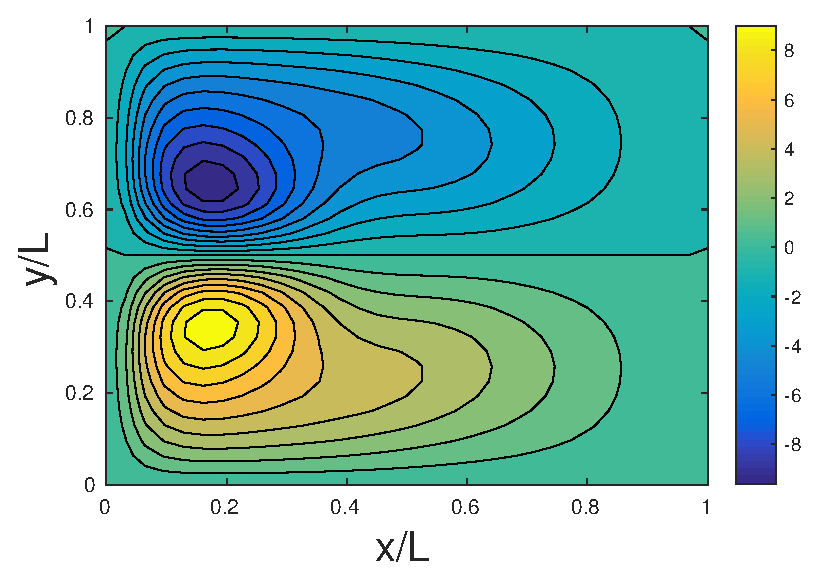
\includegraphics[width=\textwidth]{images/grid32.eps}
        \caption{$n=m=32$}
        \label{fig:nm32}
    \end{subfigure}
    ~
    \begin{subfigure}[b]{0.6\textwidth}
        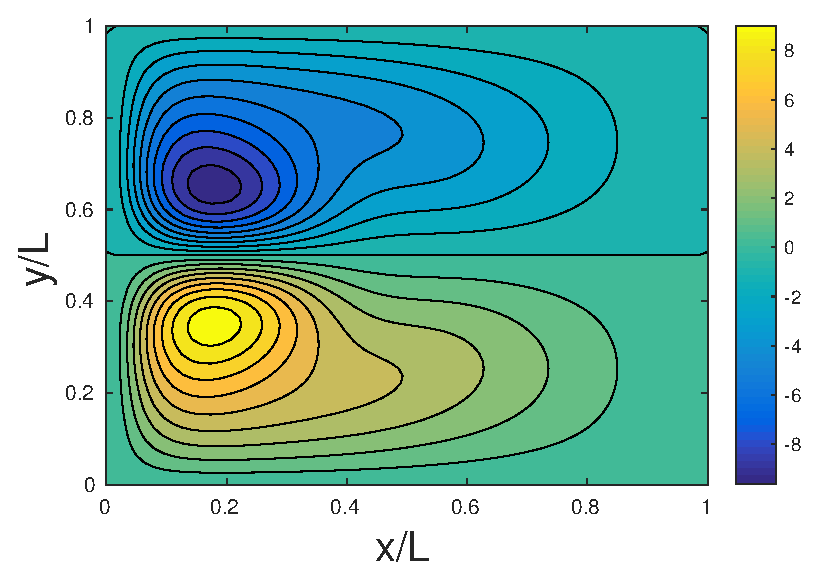
\includegraphics[width=\textwidth]{images/grid64.eps}
        \caption{$n=m=64$}
        \label{fig:nm64}
    \end{subfigure}
    }
    
    \begin{subfigure}[b]{0.6\textwidth}
        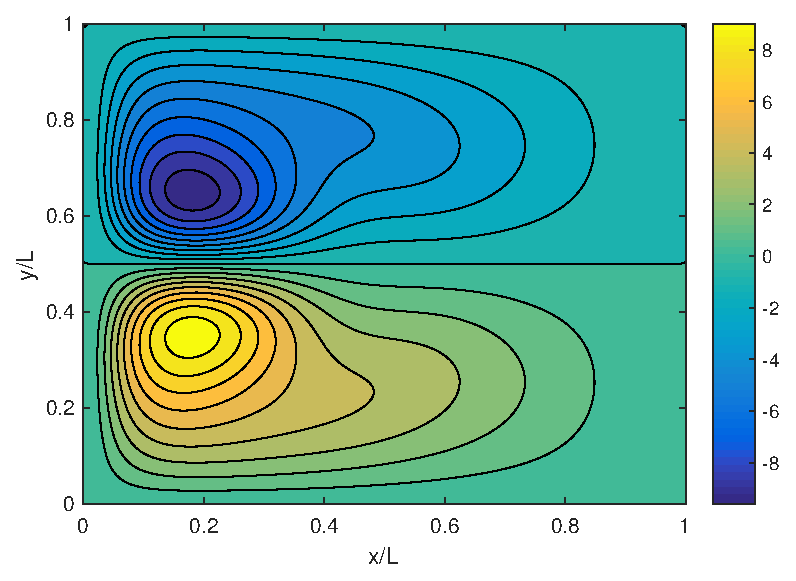
\includegraphics[width=\textwidth]{images/grid128.eps}
        \caption{$n=m=128$}
        \label{fig:nm128}
    \end{subfigure}
    
\end{figure}